\documentclass{article}
\usepackage{graphicx}
\usepackage{amsmath}
\usepackage{amsfonts}
\usepackage{geometry}
\usepackage{cite}
\usepackage{hyperref}
\geometry{a4paper, margin=1in}
\usepackage{float} % Add this to your preamble

\title{Skin Disease Detection Using the HAM1000 Dataset and Convolutional Neural Networks}
\author{Muhammad Akbar\\ Halil Ibrahim Altinbas\\
Aysegul Helal Seyhan\\
Mustafa Askan\\ }


\begin{document}

\maketitle

\begin{abstract}
Skin diseases are prevalent worldwide and pose significant health risks, both physically and mentally. The risks associated with these conditions are often not immediately visible, which can lead to distress and, in severe cases, even skin cancer. Diagnosing skin diseases from clinical images is a complex and challenging task in medical image analysis. Moreover, manual diagnosis by medical professionals is time-consuming and can be subjective. Consequently, there is a growing need for automated skin disease prediction systems to expedite treatment plans.Given the complexities involved, there is an increasing demand for highly precise computer-aided systems to aid medical practitioners in the early detection of malignant skin lesions. In this study, we propose an advanced skin lesion classification framework that integrates deep learning techniques with collective intelligence. This system leverages multiple convolutional neural networks (CNNs) trained on the HAM10000 dataset to identify seven types of skin lesions, including melanoma.
\end{abstract}

\section{Introduction}Accurate segmentation and classification of skin lesions in their early stages are vital for identifying potential malignancies. Early detection of malignant lesions significantly improves the chances of successful treatment, whereas delayed diagnosis can lead to metastasis and even death. High-precision diagnostic systems are particularly crucial for melanoma, one of the deadliest forms of skin cancer. The early identification and prevention of melanoma are therefore key concerns for medical professionals. Projections indicate that cancer rates will increase by 24.1\% in men and 20.6\% in women in the coming years [1]. Skin cancer, in particular, exhibits one of the highest annual incidence rates, with approximately 100,000 new cases reported in the United States in 2020, resulting in nearly 10,000 fatalities [2]. Although the overall mortality rate for skin cancer is relatively low (around 10\%), the treatment process is often painful, and if diagnosed too late, the condition may necessitate amputation of the affected area.

Skin cancers are generally categorized into four types: basal cell carcinoma, squamous cell carcinoma, Merkel cell carcinoma, and melanoma. Among these, melanoma is the most aggressive and lethal, accounting for the highest mortality rate. A systematic review on the use of neural network-based systems for melanoma detection was conducted in [3], underscoring the growing importance of automated tools in early diagnosis and treatment.

The HAM1000 dataset, consisting of 10,000 dermatoscopic images, serves as a benchmark for skin lesion classification. This dataset includes a diverse range of skin conditions, making it an ideal resource for training and evaluating machine learning models. In this study, we aim to leverage the HAM1000 dataset to develop a CNN model capable of accurately classifying skin lesions, thereby contributing to the field of dermatology and improving diagnostic 
 efficiency.


\newpage  % Forces a page break before the figure
\begin{figure}[h!]
    \centering
    \includegraphics[width=\textwidth]{diseases.jpg}
    \caption{Example of skin lesions used for classification.}
    \label{fig:skin_lesion_example}
\end{figure}


Many researchers have worked on skin disease classification for the last three decades. The area is so significant and has become a hot research topic. Even though many research papers are done on skin disease detection and classification, there is still a gap to be filled. Most of the previous work is based on a single disease [6], [7], and those that have been done are inadequate for classifying multiple classes [8]. The classification task of multiple classes is very challenging as the skin disease presents more similar behavior.

\section{Related Work}
\subsection{Medical Image Classification}
The application of machine learning in medical image classification has gained traction in recent years. Early approaches primarily utilized traditional machine learning algorithms, which required extensive feature engineering and domain expertise. However, these methods often struggled with generalization to unseen classes, particularly in the context of rare skin diseases.

With the advent of deep learning, CNNs have emerged as a powerful tool for image classification tasks. CNNs automatically learn hierarchical features from raw pixel data, eliminating the need for manual feature extraction. Numerous studies have demonstrated the effectiveness of CNNs in various medical imaging tasks, including skin disease detection. For instance, Esteva et al. (2017) showcased a deep learning model that achieved performance comparable to dermatologists in melanoma classification.

\subsection{The HAM1000 Dataset}
The HAM1000 dataset is a publicly available collection of dermatoscopic images, curated to facilitate research in skin lesion classification. It includes images of various skin conditions, such as melanoma, nevus, and basal cell carcinoma, along with associated metadata. The dataset is divided into training, validation, and test sets, allowing for robust model evaluation. The diversity of the dataset makes it a valuable resource for developing and benchmarking machine learning models in dermatology.

\section{Methodology}
\subsection{Dataset Overview}
The HAM1000 dataset consists of 10,000 images, each labeled with one of seven skin lesion categories: melanoma, nevus, basal cell carcinoma, actinic keratosis, dermatofibroma, vascular lesions, and seborrheic keratosis. The images vary in size, resolution, and quality, necessitating preprocessing to ensure uniformity.



\section{Existing Methods}

Recent research in the field of skin lesion detection has shown a growing trend toward using a combination of various techniques and deep learning models to achieve higher accuracy and better generalization. Many of these systems leverage multiple classifiers and deep convolutional neural networks (CNNs) in different architectures to tackle the challenges posed by skin lesion classification.

\subsection{Combination of ABCDE with Support Vector Machine (SVM)}
Some studies have explored combining traditional techniques such as the ABCDE rule (Asymmetry, Border, Color, Diameter, and Evolution) with machine learning classifiers like SVM to improve classification accuracy. This hybrid approach often capitalizes on the robustness of traditional heuristics and the power of machine learning models.

\subsection{Transfer Learning and Modified Networks}
Another common strategy is the use of modified neural networks, particularly with transfer learning. This method involves fine-tuning pre-trained models on skin lesion datasets to adapt them to the specific task of lesion detection. By leveraging the knowledge embedded in large models, researchers have been able to achieve promising results in skin lesion classification \cite{Popescu2022}.

\subsection{Multiple Networks and Ensemble Models}
Multiple networks are also employed in an ensemble fashion, where each model contributes a part to the overall system's decision. For example, one network may perform lesion segmentation while another takes over the classification task using the segmented data. This approach is particularly effective in dealing with complex datasets where different aspects of the image (e.g., color, shape, texture) need to be considered for accurate diagnosis. Ensemble models like these have been found to outperform single networks in terms of accuracy and robustness \cite{Esteva2017, Akram2020}.

\subsection{Pre-trained Networks for Feature Extraction}
Convolutional neural networks (CNNs) such as AlexNet, ResNet, and GoogLeNet have been widely adopted for their excellent feature extraction capabilities. These models are trained on large datasets and fine-tuned for skin lesion classification. For instance, Esteva et al. \cite{Esteva2017} used GoogLeNet Inception-V3 to achieve dermatologist-level classification of skin cancer, showing its effectiveness in the domain. AlexNet, though older, has still shown strong performance, achieving an accuracy of 93.64\% in some skin mole detection systems \cite{Pomponiu2016}.

\subsection{Residual Networks (ResNet) and Deep Learning}
As CNNs have become deeper, the issue of vanishing gradients has prompted the use of residual networks like ResNet-50 and ResNet-101. These architectures help improve the accuracy of deep models by allowing gradients to flow more effectively through the network. Studies have demonstrated the use of ResNet-50 in melanoma classification, with accuracy reaching up to 90.67\% when combined with handcrafted features \cite{Almaraz-Damian2020}. Similar success has been seen with networks like Xception and MobileNet-V2, which are also frequently applied in skin lesion diagnosis due to their lightweight and efficient architecture \cite{Almaraz-Damian2020}.

\subsection{DenseNet and Feature Fusion}
DenseNet-201 is another frequently used architecture, especially for feature extraction and classification. Research has combined DenseNet-201 with fully convolutional networks for segmentation, achieving up to 81.29\% accuracy on the ISIC 2017 dataset \cite{Al-masni2020}. This model benefits from its densely connected layers, which improve feature reuse and facilitate learning.

\subsection{Hybrid Models for Skin Disease Classification}
Hybrid models that combine different architectures and classifiers have shown promise in tackling a range of skin diseases. For example, a multi-class system combining ResNet, AlexNet, and other CNN models has been proposed to classify various types of skin lesions, including melanoma, using ensemble voting systems to enhance prediction accuracy \cite{Ichim2020}.

\subsection{Decision Fusion and Voting Systems}
Researchers have also developed complex voting systems that combine the outputs of several models. These systems typically rely on the outputs from multiple CNNs trained for different tasks (e.g., melanoma vs. non-melanoma classification) and aggregate the results using a decision-making process like majority voting or confidence-weighted averaging. One such example is the multi-network voting system proposed by Gong et al. \cite{Gong2020}, which combines the strengths of various individual networks for accurate lesion classification.

In conclusion, the trend in skin lesion classification is moving towards \textbf{ensemble models}, \textbf{transfer learning}, and \textbf{multi-network systems} that aim to leverage the strengths of multiple techniques to achieve higher accuracy and robustness. This approach is expected to remain a significant direction in future research, particularly with the continuous evolution of neural network architectures and the availability of larger and more diverse datasets.


\section{Materials}

3.1. Dataset Used
There are many datasets with skin lesions: PH2, ISIC 2016, ISIC 2017, ISIC 2018-HAM10000, ISIC 2019, ISIC 2020, DERMQUEST, MED-NODE, DERMNET, DERMIS, DERMOFIT, etc. [3]. HAM10000 is one of the largest skin lesions datasets publicly available for academic research. In this paper, for current experiments, we chose to use the HAM10000 (“Human Against Machine with 10,000 training images”) dataset, introduced in the ISIC 2018 challenge, which contains 10,015 dermatoscopic images which can serve as a training dataset for academic machine learning purposes [6]. The HAM10000 dataset covers image samples for all-important diagnostic categories (classes) in the real pigmented lesions:

Actinic keratoses and intraepithelial carcinoma/Bowen’s disease (akiec)

Basal cell carcinoma (bcc)

Benign keratosis-like lesions (bkl-solar lentigines/seborrheic keratoses and lichen-planus like keratoses)

Dermatofibroma (df)

Melanoma (mel)

Melanocytic nevi (nv)

Vascular lesions (vasc-angiomas, angiokeratomas, pyogenic granulomas, and hemorrhage).

HAM10000 dataset contains 1015 JPEG images and is split into two packages/folders: \text{HAM10000\_imagespart1} (5000 JPEG images) and \text{HAM10000\_imagespart2} (5015 JPEG images). Some examples are presented below in Figure 1



\begin{figure}[htbp]
\centering
\includegraphics[width=\textwidth, angle=0]{tileshop.jpg}  % Adjusts the width of the image to fit the page, angle=0 means no rotation
\caption{Example of each class from HAM10000 dataset }


\label{fig:your_label}
\end{figure}


\subsection{Data Preprocessing}
Before training the CNN model, we perform several preprocessing steps:
% \begin{itemize}
    \item \textbf{Image Resizing:} All images are resized to different uniform dimension (e.g., 224x224, 56,56 pixels) to ensure compatibility with different types of models in CNN architecture.
    \item \textbf{Normalization:} Pixel values are normalized to a range of [0, 1] to improve convergence during training.
    \item \textbf{Data Augmentation:} To enhance the model's robustness and prevent overfitting, we apply data augmentation techniques, including random rotations, flips, and brightness adjustments. This increases the diversity of the training dataset without the need for additional labeled data. Data augmentation can be useful in the training phase if the data in certain classes of the dataset is small. This can reduce the overfitting of the deep neural networks. 
    all of this occurs in the part 
 
We used dataset augmentation methods to try to balance the data (classes). As can be seen in Figure 2, the following augmentation methods were applied:



\begin{figure}[h!]
    \centering
    \includegraphics[width=\textwidth]{aug.jpg}
    \caption{Vertical or horizontal pixel shift with a maximum of 10
.}
    \label{fig:skin_lesion_example}
\end{figure}


% \end{itemize}

\section{CNN Architecture}

In this study, we explore the use of Convolutional Neural Networks (CNNs) for skin disease detection using the **HAM10000 dataset**. We evaluate and compare two different approaches to build the model architecture: a single CNN model and different ready made image classification models from keras. Each approach has distinct advantages, and their implementation is discussed below.

\subsection{Standard CNN Model}

The standard CNN model is a single deep learning network that is typically trained from scratch or fine-tuned using a pre-trained model on a large dataset like ImageNet. The goal of the CNN model is to automatically extract features from input images through layers of convolutions, pooling, and fully connected layers to classify the data.

\subsubsection{Architecture of the Standard CNN Model}

The architecture of the standard CNN model follows a typical design pattern:
\begin{itemize}
    \item \textbf{Input Layer:} The input to the model is an image with a fixed size, typically 224x224 or 256x256 pixels, and 3 color channels (RGB) but due to limited resources i have used 58x58 pixel images in my CNN model.
    \item \textbf{Convolutional Layers:} The convolutional layers apply various filters to the input images, extracting hierarchical features like edges, textures, and shapes. These layers are followed by activation functions (e.g., ReLU) to introduce non-linearity.
    \begin{figure}[H]
    \centering
    \includegraphics[width=0.45 \textwidth]{conv.png}
    \caption{Illustration of convolutional layers extracting features.}
    \label{fig:conv_layer}
\end{figure}

    \item \textbf{Pooling Layers:} After the convolutional layers, pooling layers (usually MaxPooling) reduce the spatial dimensions of the feature maps, making the model more computationally efficient while preserving important information.  \begin{figure}[h]
    \centering
    \includegraphics[width=0.45 \textwidth]{maxpool.png}
    \caption{Illustration of a functioning Max Pooling layer.}
    \label{fig:conv_layer}
\end{figure}

    
    \item \textbf{Fully Connected Layers:} After the feature extraction layers, the output is flattened and passed through fully connected (dense) layers. These layers are used to combine the features learned from the previous layers and make the final prediction.
      \begin{figure}[H]
    \centering
    \includegraphics[width=0.45 \textwidth]{fullyConectedLayer.png}
    \caption{Fully COnnected Layer.}
    \label{fig:conv_layer}
\end{figure}

    \item \textbf{Output Layer:} The output layer uses a softmax activation function for multi-class classification. Each class corresponds to a specific skin disease type, and the network outputs a probability distribution for each class.
        \begin{figure}[H]
    \centering
    \includegraphics[width=0.45 \textwidth]{output.png}
    \caption{All Layers  performing to give results that contribute in predicting the class using output layer.}
    \label{fig:conv_layer}
\end{figure}

\end{itemize}

\subsubsection{Advantages of the Standard CNN Model}

The standard CNN model has several advantages:
\begin{itemize}
    \item It is straightforward to implement and train on a given dataset.
    \item Automatic feature extraction.
    \item Highly accurate at image recognition & classification.
(although our model may have some tendency to not show 100\% performance but that is absolutely not because the structure of cnn lacks ability or the algorithm is faulty)
    
    \item It requires fewer resources compared to more complex architectures like ensemble models.
    \item   their ability to perform automatic feature extraction or feature learning. 
\end{itemize}

However, the model's performance is limited by its single architecture, which may not capture all the complex features of the dataset, leading to overfitting or reduced accuracy on unseen data.

\subsection{Famous CNN  Models}

Apart from this CNN model we are building from scratch, we will make  use of and analyse different ready made CNN models on our HAM1000 dataset to discover abilities and weaknesses of different algorithms
\subsubsection{Architecture of different models}

For the sake of our project, we shall perform detailed analysis of impact of different ready made models on several pre-trained CNN models, such as \textbf{ResNet50}, \textbf{VGG16}, and \textbf{DenseNet}, to form a stronger classifier. Each model is trained independently, and their predictions are combined to improve accuracy.
\section{Detailed Architecture of CNN Models}

\subsection{VGG16}
\textbf{VGG16} is a deep convolutional neural network that has 16 layers with weights. It follows a simple and uniform architecture, using only $3\times3$ convolutional filters and $2\times2$ max-pooling layers.
\begin{itemize}
    \item \textbf{Input Layer:} Accepts an input image of size $224\times224\times3$ (RGB image).
    \item \textbf{Convolutional Layers:} 
    \begin{itemize}
        \item Consists of 13 convolutional layers.
        \item All convolutional layers use $3\times3$ filters with a stride of 1 and padding to preserve the spatial resolution.
    \end{itemize}
    \item \textbf{Pooling Layers:} 
    \begin{itemize}
        \item 5 max-pooling layers with a filter size of $2\times2$ and stride of 2.
        \item These layers downsample the spatial dimensions progressively.
    \end{itemize}
    \item \textbf{Fully Connected Layers:}
    \begin{itemize}
        \item 3 fully connected layers.
        \item The first two layers have 4096 neurons each, followed by an output layer with 1000 neurons (for ImageNet classification).
    \end{itemize}
    \item \textbf{Activation Function:} Uses ReLU after each convolutional and fully connected layer.
    \item \textbf{Output Layer:} A softmax activation function to output probabilities for each class.

    information.  \begin{figure}[H]
    \centering
    \includegraphics[width=0.45 \textwidth]{vgg16.png}
    \caption{VGG16 Architecture.}
    \label{fig:conv_layer}
\end{figure}

\end{itemize}

\subsection{ResNet (Residual Networks)}
\textbf{ResNet} introduces the concept of residual connections to solve the vanishing gradient problem in deep networks. The ResNet architecture has several variations, such as ResNet-18, ResNet-34, ResNet-50, ResNet-101, and ResNet-152.
\begin{itemize}
    \item \textbf{Input Layer:} Accepts an input image of size $224\times224\times3$.
    \item \textbf{Convolutional Layers:} 
    \begin{itemize}
        \item Initial $7\times7$ convolutional layer with a stride of 2.
        \item Subsequent layers use $3\times3$ or $1\times1$ filters in residual blocks.
    \end{itemize}
    \item \textbf{Residual Blocks:} 
    \begin{itemize}
        \item Consist of shortcut (skip) connections that bypass one or more layers.
        \item Each block has a series of convolutions, batch normalization, and ReLU activations.
    \end{itemize}
    \item \textbf{Pooling Layers:} Includes both max-pooling and global average pooling layers.
    \item \textbf{Fully Connected Layer:} A single dense layer that outputs 1000 classes.
    \item \textbf{Activation Function:} ReLU after each convolution.
    \item \textbf{Output Layer:} A softmax activation function.

    information.  \begin{figure}[H]
    \centering
    \includegraphics[width=0.45 \textwidth]{resnet.png}
    \caption{resnet Architecture.}
    \label{fig:conv_layer}
\end{figure}

\end{itemize}

\subsection{DenseNet (Dense Convolutional Networks)}
\textbf{DenseNet} connects each layer to every other layer in a feed-forward fashion. This architecture improves parameter efficiency and feature reuse.
\begin{itemize}
    \item \textbf{Input Layer:} Accepts an input image of size $224\times224\times3$.
    \item \textbf{Dense Blocks:} 
    \begin{itemize}
        \item Each block contains multiple layers, with each layer taking inputs from all preceding layers.
        \item Uses batch normalization, ReLU activation, and $3\times3$ convolutional filters.
    \end{itemize}
    \item \textbf{Transition Layers:}
    \begin{itemize}
        \item Positioned between dense blocks.
        \item Includes $1\times1$ convolutional layers and $2\times2$ average pooling layers to reduce dimensions.
    \end{itemize}
    \item \textbf{Fully Connected Layer:} Outputs class probabilities.
    \item \textbf{Activation Function:} ReLU after each convolution.
    \item \textbf{Output Layer:} A softmax activation function.

     \begin{figure}[H]
    \centering
    \includegraphics[width=0.45 \textwidth]{densenet.png}
    \caption{densenet Architecture.}
    \label{fig:conv_layer}
\end{figure}

\end{itemize}


\end{itemize}

% \subsubsection{Advantages of the Ensemble Learning Model}

% The ensemble learning model has several benefits:
% \begin{itemize}
%     \item It reduces the risk of overfitting by combining the predictions of multiple models, making it more robust to noise in the data.
%     \item The ensemble model captures diverse features from each base model, leading to a more comprehensive understanding of the data.
%     \item It typically achieves higher accuracy compared to a single model, especially when the models in the ensemble are complementary to each other.
% \end{itemize}

% However, ensemble learning has its drawbacks:
% \begin{itemize}
%     \item It requires more computational resources and time for both training and inference.
%     \item It is more complex to implement and maintain due to the integration of multiple models.
% \end{itemize}

% \subsection{Comparison of Standard CNN and Ensemble Learning Models}

% While both the standard CNN and ensemble learning approaches can be applied for skin disease detection, there are key differences in their performance, training time, and generalization capabilities.

% \subsubsection{Performance Comparison}

% Ensemble learning tends to outperform a single CNN model in terms of accuracy, as it combines the strengths of different models. Each model in the ensemble may capture different aspects of the data, resulting in a more robust and accurate prediction. On the other hand, the standard CNN model, though effective, may have limitations in capturing all the complexities of the data, leading to lower generalization performance.

% \subsubsection{Training Time and Complexity}

% Training an ensemble model is significantly more time-consuming than training a single CNN model due to the need to train multiple base models. Moreover, ensemble models require more computational resources during inference, as predictions must be aggregated from several models. In contrast, the standard CNN model is simpler, faster, and less resource-intensive, making it more suitable for applications where computational resources are limited.

% \subsubsection{Overfitting and Generalization}

% Ensemble learning generally offers better generalization compared to a single CNN model, particularly when the dataset is small or noisy. By combining predictions from multiple models, the ensemble reduces the chance of overfitting and improves the model’s ability to handle unseen data. The standard CNN model, while effective, is more prone to overfitting, especially if the dataset is not large enough or if the model architecture is too complex.



\subsection{Training Procedure for Standard CNN Model}

The training procedure for the standard CNN model follows the typical setup for deep learning models. Below are the key training parameters:

\begin{itemize}
    \item \textbf{Batch Size:} We utilize a batch size of 32, which strikes a balance between memory efficiency and convergence speed. This allows the model to process 32 images simultaneously, updating the weights based on the average loss across the batch.
    \item \textbf{Optimizer:} The Adam optimizer is employed for training. It starts with a learning rate of 0.001 and later adapts the learning rate for each parameter based on the first and second moments of the gradients. This helps in achieving faster convergence and better performance.

The Adam optimizer combines the advantages of two other extensions of stochastic gradient descent: AdaGrad and RMSprop. It computes adaptive learning rates for each parameter by considering both the mean and the uncentered variance of the gradients.

The update rule for Adam is as follows:
\[
m_t = \beta_1 m_{t-1} + (1 - \beta_1) g_t
\]
\[
v_t = \beta_2 v_{t-1} + (1 - \beta_2) g_t^2
\]
\[
\hat{m}_t = \frac{m_t}{1 - \beta_1^t}
\]
\[
\hat{v}_t = \frac{v_t}{1 - \beta_2^t}
\]
\[
\theta_t = \theta_{t-1} - \frac{\eta}{\sqrt{\hat{v}_t} + \epsilon} \hat{m}_t
\]
Where:
\begin{itemize}
    \item \( m_t \) and \( v_t \) are the first and second moment estimates (mean and variance of gradients),
    \item \( g_t \) is the gradient at time step \( t \),
    \item \( \beta_1 \) and \( \beta_2 \) are the exponential decay rates for the first and second moment estimates (usually set to 0.9 and 0.999, respectively),
    \item \( \eta \) is the learning rate,
    \item \( \epsilon \) is a small constant to prevent division by zero (typically set to \( 10^{-8} \)),
    \item \( \hat{m}_t \) and \( \hat{v}_t \) are bias-corrected estimates.
\end{itemize}
\item \textbf{Loss Function:} Sparse categorical cross-entropy is used as the loss function, which is suitable for multi-class classification problems with integer-encoded labels. This function measures the dissimilarity between the predicted probability distribution and the true distribution of the labels.

The formula for sparse categorical cross-entropy is given by:
\[
L = - \sum_{i=1}^{N} y_i \log(p_i)
\]
Where:
\begin{itemize}
    \item \( L \) is the loss,
    \item \( N \) is the number of classes,
    \item \( y_i \) is the true label (integer-encoded, i.e., an integer representing the correct class),
    \item \( p_i \) is the predicted probability for the \( i \)-th class,
    \item The sum is taken over all classes.
\end{itemize}

In this formula, the loss penalizes the predicted probabilities \( p_i \) for the incorrect classes more heavily, encouraging the model to output higher probabilities for the correct class. The lower the loss, the better the model's predictions match the true labels.

    \item \textbf{Training Epochs:} The model is trained for a predetermined number of epochs (e.g., 15), with early stopping implemented to prevent overfitting. The validation set is monitored during training, and if the validation loss does not improve for a specified number of epochs, training is halted to prevent overfitting and save resources.
\end{itemize}




\subsection{Training Procedure for VGG16  Model}

\begin{itemize}
    \item \textbf{Batch Size:} We utilize a batch size of 10, which strikes a balance between memory efficiency and convergence speed. This allows the model to process 10 images simultaneously, updating the weights based on the average loss across the batch.
    \item \textbf{Optimizer:} \item \textbf{RMSprop:} RMSprop (Root Mean Square Propagation) is an adaptive learning rate optimization algorithm. It adjusts the learning rate for each parameter based on the magnitude of recent gradients. It helps to reduce the impact of large gradients and improves convergence in situations with noisy or sparse gradients.

The formula for RMSprop is as follows:
\[
v_t = \beta v_{t-1} + (1 - \beta) g_t^2
\]
\[
\theta_t = \theta_{t-1} - \frac{\eta}{\sqrt{v_t + \epsilon}} g_t
\]
Where:
\begin{itemize}
    \item \( v_t \) is the running average of the squared gradients,
    \item \( \beta \) is the decay factor (usually close to 1, e.g., 0.9),
    \item \( g_t \) is the gradient at time step \( t \),
    \item \( \eta \) is the learning rate,
    \item \( \epsilon \) is a small constant to prevent division by zero.
\end{itemize}
RMSprop helps in maintaining a steady and adaptive learning rate, particularly in problems where the gradient can vary in scale.

  \item \textbf{Loss Function:}\item \textbf{Categorical Cross-Entropy:} Categorical cross-entropy is a loss function used for multi-class classification problems, where each label is one-hot encoded. It measures the dissimilarity between the predicted probability distribution and the true distribution of the labels.

The formula for categorical cross-entropy is given by:
\[
L = - \sum_{i=1}^{N} y_i \log(p_i)
\]
Where:
\begin{itemize}
    \item \( L \) is the loss,
    \item \( N \) is the number of classes,
    \item \( y_i \) is the true label (one-hot encoded, i.e., 1 for the correct class and 0 for the others),
    \item \( p_i \) is the predicted probability for the \( i \)-th class,
    \item The sum is taken over all classes.
\end{itemize}

In this formula, the loss penalizes the predicted probabilities \( p_i \) for the incorrect classes more heavily, encouraging the model to output higher probabilities for the correct class. The lower the loss, the better the model's predictions match the true labels.


    \item \textbf{Training Epochs:} The model is trained for a predetermined number of epochs (e.g., 10), with early stopping implemented to prevent overfitting. The validation set is monitored during training, and if the validation loss does not improve for a specified number of epochs, training is halted to prevent overfitting and save resources.
\end{itemize}

\subsection{Training Procedure for ResNet Model}

\begin{itemize}
    \item \textbf{Batch Size:} We utilize a batch size of 32, which is a standard choice for ResNet models. This batch size ensures efficient processing while maintaining an adequate memory footprint for training.
    \item \textbf{Optimizer:} \item \textbf{Adam:} Adam (Adaptive Moment Estimation) is used as the optimizer for ResNet. Adam adjusts the learning rate for each parameter based on the first and second moments of the gradients, leading to faster convergence and better performance.

    The update rule for Adam is as follows:
    \[
    m_t = \beta_1 m_{t-1} + (1 - \beta_1) g_t
    \]
    \[
    v_t = \beta_2 v_{t-1} + (1 - \beta_2) g_t^2
    \]
    \[
    \hat{m}_t = \frac{m_t}{1 - \beta_1^t}
    \]
    \[
    \hat{v}_t = \frac{v_t}{1 - \beta_2^t}
    \]
    \[
    \theta_t = \theta_{t-1} - \frac{\eta}{\sqrt{\hat{v}_t} + \epsilon} \hat{m}_t
    \]
    Where:
    \begin{itemize}
        \item \( m_t \) and \( v_t \) are the first and second moment estimates (mean and variance of gradients),
        \item \( g_t \) is the gradient at time step \( t \),
        \item \( \beta_1 \) and \( \beta_2 \) are the exponential decay rates for the first and second moment estimates (usually set to 0.9 and 0.999),
        \item \( \eta \) is the learning rate,
        \item \( \epsilon \) is a small constant to prevent division by zero.
    \end{itemize}
    \item \textbf{Loss Function:} \item \textbf{Categorical Cross-Entropy:} Categorical cross-entropy is used as the loss function for multi-class classification. It compares the predicted probability distribution with the true distribution of one-hot encoded labels.

    The formula for categorical cross-entropy is:
    \[
    L = - \sum_{i=1}^{N} y_i \log(p_i)
    \]
    Where:
    \begin{itemize}
        \item \( L \) is the loss,
        \item \( N \) is the number of classes,
        \item \( y_i \) is the true label (one-hot encoded),
        \item \( p_i \) is the predicted probability for the \( i \)-th class.
    \end{itemize}
    \item \textbf{Training Epochs:} The model is trained for a fixed number of epochs (e.g., 20), with early stopping based on validation performance to prevent overfitting.
\end{itemize}

\subsection{Training Procedure for DenseNet Model}

\begin{itemize}
    \item \textbf{Batch Size:} A batch size of 16 is chosen to manage memory requirements and convergence speed. DenseNet models, due to their dense connections, may require slightly smaller batch sizes.
    \item \textbf{Optimizer:} \item \textbf{Adam:} The Adam optimizer is used for DenseNet. Adam adapts the learning rate for each parameter by using the first and second moments of the gradients, helping DenseNet achieve faster convergence.

    The update rule for Adam is:
    \[
    m_t = \beta_1 m_{t-1} + (1 - \beta_1) g_t
    \]
    \[
    v_t = \beta_2 v_{t-1} + (1 - \beta_2) g_t^2
    \]
    \[
    \hat{m}_t = \frac{m_t}{1 - \beta_1^t}
    \]
    \[
    \hat{v}_t = \frac{v_t}{1 - \beta_2^t}
    \]
    \[
    \theta_t = \theta_{t-1} - \frac{\eta}{\sqrt{\hat{v}_t} + \epsilon} \hat{m}_t
    \]
    Where:
    \begin{itemize}
        \item \( m_t \) and \( v_t \) are the first and second moment estimates,
        \item \( g_t \) is the gradient at time \( t \),
        \item \( \beta_1 \) and \( \beta_2 \) are the decay rates,
        \item \( \eta \) is the learning rate,
        \item \( \epsilon \) is a small constant.
    \end{itemize}
    \item \textbf{Loss Function:} \item \textbf{Categorical Cross-Entropy:} The loss function for DenseNet is categorical cross-entropy, suitable for multi-class classification.

    The formula is:
    \[
    L = - \sum_{i=1}^{N} y_i \log(p_i)
    \]
    Where:
    \begin{itemize}
        \item \( L \) is the loss,
        \item \( N \) is the number of classes,
        \item \( y_i \) is the true label,
        \item \( p_i \) is the predicted probability for the \( i \)-th class.
    \end{itemize}
    \item \textbf{Training Epochs:} DenseNet is trained for 30 epochs, with early stopping based on validation accuracy to avoid overfitting.
\end{itemize}

\subsection{Training Procedure for MobileNet Model}

\begin{itemize}
    \item \textbf{Batch Size:} A batch size of 64 is chosen for MobileNet. This larger batch size helps in faster training while maintaining an efficient memory footprint.
    \item \textbf{Optimizer:} \item \textbf{RMSprop:} RMSprop is the optimizer used for training MobileNet. It adjusts the learning rate for each parameter based on the average squared gradients, which helps in situations with noisy gradients.

    The formula for RMSprop is:
    \[
    v_t = \beta v_{t-1} + (1 - \beta) g_t^2
    \]
    \[
    \theta_t = \theta_{t-1} - \frac{\eta}{\sqrt{v_t + \epsilon}} g_t
    \]
    Where:
    \begin{itemize}
        \item \( v_t \) is the running average of squared gradients,
        \item \( \beta \) is the decay factor (typically set to 0.9),
        \item \( g_t \) is the gradient at time step \( t \),
        \item \( \eta \) is the learning rate,
        \item \( \epsilon \) is a small constant for numerical stability.
    \end{itemize}
    \item \textbf{Loss Function:} \item \textbf{Sparse Categorical Cross-Entropy:} Sparse categorical cross-entropy is used for MobileNet, suitable for integer-encoded labels in multi-class classification problems.

    The formula for sparse categorical cross-entropy is:
    \[
    L = - \sum_{i=1}^{N} y_i \log(p_i)
    \]
    Where:
    \begin{itemize}
        \item \( L \) is the loss,
        \item \( N \) is the number of classes,
        \item \( y_i \) is the true label (integer-encoded),
        \item \( p_i \) is the predicted probability for the \( i \)-th class.
    \end{itemize}
    \item \textbf{Training Epochs:} MobileNet is trained for 15 epochs with early stopping to avoid overfitting, monitoring validation accuracy.
\end{itemize}

\subsection{Training Procedure for Ensemble Learning Model}

The training procedure for the ensemble learning model follows a similar setup to the standard CNN model, but with additional complexity due to the multiple base models. In our ensemble model, we leverage several pre-trained models to capture diverse learning patterns, including:

\begin{itemize}
   
    \item \textbf{ResNet-50 (NN4, df, C4)}
    \item \textbf{MobileNet-V2 (NN7, vasc, C7)}
    \item \textbf{DenseNet-201 (NN8)}
\end{itemize}

Below are the key training parameters for this ensemble model:

\begin{itemize}
    \item \textbf{Batch Size:} We utilize a batch size of 32, similar to the standard CNN model, to balance memory efficiency and convergence speed. This allows the ensemble model to process 32 images in parallel, updating the weights of each individual base model based on the average loss across the batch.
    \item \textbf{Optimizer:} The Adam optimizer is also employed for each base model within the ensemble. It adapts the learning rate for each parameter based on the first and second moments of the gradients, helping each model achieve faster convergence and better performance during training.
    \item \textbf{Loss Function:} Categorical cross-entropy is used as the loss function for each base model. As the ensemble involves multiple models, each model calculates its loss independently, and the final prediction is obtained by combining the outputs of these models.
    \item \textbf{Training Epochs:} The ensemble model is trained for a predetermined number of epochs (e.g., 50), with early stopping implemented for each base model to prevent overfitting. The validation set is monitored for each individual model, and if a model's validation loss does not improve for a specified number of epochs, training for that model is halted. The ensemble as a whole is evaluated by combining the outputs from all trained base models.
\end{itemize}

\section{Evaluation Metrics}

To assess the performance of the trained models, we utilize several evaluation metrics. These metrics help us quantify how well the models perform in classifying skin diseases. We present the evaluation metrics for both the normal CNN model and the ensemble learning model below.
\section*{Evaluation Metrics}

\subsection*{1. Precision}  
\textbf{Definition:} Precision measures the proportion of true positive predictions among all positive predictions. It indicates the model's ability to avoid false positives.  
\[
\section*{Evaluation Metrics}

\subsection*{1. Precision}  
\textbf{Definition:} Precision measures the proportion of true positive predictions among all positive predictions. It indicates the model's ability to avoid false positives.  
\[
\text{Precision} = \frac{TP}{TP + FP}
\]

\subsection*{2. Recall (Sensitivity)}  
\textbf{Definition:} Recall, also known as Sensitivity or True Positive Rate, measures the proportion of actual positives that were correctly identified. It evaluates the model's ability to detect positive samples.  
\[
\text{Recall} = \frac{TP}{TP + FN}
\]

\subsection*{3. Accuracy}  
\textbf{Definition:} Accuracy measures the proportion of correctly classified samples out of the total samples. It provides an overall performance measure of the model.  
\[
\text{Accuracy} = \frac{TP + TN}{TP + TN + FP + FN}
\]

\subsection*{4. F1-Score}  
\textbf{Definition:} F1-Score is the harmonic mean of Precision and Recall. It balances the trade-off between Precision and Recall, especially useful for imbalanced datasets.  
\[
F1 = 2 \cdot \frac{\text{Precision} \cdot \text{Recall}}{\text{Precision} + \text{Recall}}
\]

\section{Implementation}

In this section, we present the results obtained from different deep learning models for skin disease classification, focusing on precision, accuracy, and recall. We evaluate the performance of the following models: a standard Convolutional Neural Network (CNN), VGG16, ResNet, and DenseNet. The evaluation is performed using precision, recall, and accuracy metrics on both the training and validation datasets.

\subsection{CNN Model}
The standard CNN model achieved an accuracy of 0.9997 on the training data, indicating that it is highly effective in learning the features necessary for skin disease classification. Below are the training results:

\[
\text{Accuracy (Training):} \quad 0.9997
\]
\[
\text{Precision (Training):} \quad 0.9818
\]
\[
\text{Recall (Training):} \quad 0.1049
\]

These values suggest that the CNN model has a high precision, meaning that most positive predictions it makes are correct. However, the recall is relatively low, indicating that the model fails to identify many instances of the disease. This issue could be attributed to the class imbalance in the dataset, where positive samples are less frequent or the model is overly tuned to avoid false positives, thus missing many true positives.

On the validation set, the model performed as follows:

\[
\text{Accuracy (Validation):} \quad 0.9818
\]
\[
\text{Loss (Validation):} \quad 0.1049
\]

Although the accuracy and loss on the validation set are high, the model could still benefit from techniques like data augmentation or using more advanced regularization methods to improve recall.

\subsection{VGG16}
VGG16, a deeper architecture than the standard CNN, achieved a training accuracy of 0.7221, as shown below:

\[
\text{Accuracy (Training):} \quad 0.7221
\]
\[
\text{Precision (Training):} \quad 0.8281
\]
\[
\text{Recall (Training):} \quad 0.6190
\]

Despite the drop in accuracy compared to CNN, VGG16 has a higher recall, which means it identifies more true positive cases. However, the precision is lower than that of the CNN model, suggesting that VGG16 generates more false positives.

On the validation set, the results are:

\[
\text{Accuracy (Validation):} \quad 0.6833
\]
\[
\text{Loss (Validation):} \quad 14.9488
\]
\[
\text{Precision (Validation):} \quad 0.6833
\]
\[
\text{Recall (Validation):} \quad 0.6833
\]

The validation results show that VGG16 experiences overfitting, as evidenced by a significant drop in accuracy and an unusually high loss value. This overfitting could be caused by insufficient regularization or a lack of variety in the training data.

\subsection{ResNet}
ResNet, with its residual connections, performs better than VGG16 in terms of precision. The training results are:

\[
\text{Accuracy (Training):} \quad 0.6756
\]
\[
\text{Precision (Training):} \quad 0.8209
\]
\[
\text{Recall (Training):} \quad 0.5767
\]

These values show that while ResNet has a relatively high precision, it misses some disease instances (lower recall). This can be attributed to the model's ability to focus more on correctly classified samples (high precision) but not generalizing well to rare disease cases (low recall).

On the validation set, the results are as follows:

\[
\text{Accuracy (Validation):} \quad 0.7082
\]
\[
\text{Loss (Validation):} \quad 0.8375
\]
\[
\text{Precision (Validation):} \quad 0.9130
\]
\[
\text{Recall (Validation):} \quad 0.5362
\]

The high precision on the validation set suggests that ResNet performs well in detecting positive cases, but its recall remains lower, indicating that there is still a gap in identifying all instances of the disease. This could be due to insufficient data, or the model might need further fine-tuning to improve recall.

\subsection{DenseNet}
DenseNet, which encourages feature reuse and helps alleviate vanishing gradient issues, achieved the following training results:

\[
\text{Accuracy (Training):} \quad 0.8233
\]
\[
\text{Precision (Training):} \quad 0.8490
\]
\[
\text{Recall (Training):} \quad 0.7328
\]

DenseNet shows the best overall performance with higher recall, indicating that it captures more true positive samples than the other models. This could be attributed to the dense connections that allow the model to learn more robust features. The precision is also high, reflecting that the model makes fewer false-positive predictions.

For the validation set, DenseNet produced the following results:

\[
\text{Accuracy (Validation):} \quad 0.7618
\]
\[
\text{Loss (Validation):} \quad 0.7584
\]
\[
\text{Precision (Validation):} \quad 0.8146
\]
\[
\text{Recall (Validation):} \quad 0.6409
\]

These results show that DenseNet performs well on the validation set, achieving a good balance of precision and recall. Although its precision is slightly lower than the training set, it still outperforms the other models in both accuracy and recall, making it the most promising model in this study.

\begin{table}[h!]
\centering
\begin{tabular}{|l|c|c|c|}
\hline
\textbf{Model} & \textbf{Accuracy} & \textbf{Precision} & \textbf{Recall} \\
\hline
Standard CNN & 0.9997 & 0.9818 & 0.1049 \\
\hline
VGG16 & 0.7221 & 0.8281 & 0.6190 \\
\hline
ResNet & 0.6756 & 0.8209 & 0.5767 \\
\hline
DenseNet & 0.8233 & 0.8490 & 0.7328 \\
\hline
\end{tabular}
\caption{Comparison of Model Performance on Precision, Accuracy, and Recall}
\end{table}

\section{Limitations of Ensemble Models on HAM10000 Dataset}

Ensemble learning, which combines predictions from multiple models to improve performance, is often employed to boost accuracy and robustness in classification tasks. However, its application to the HAM10000 dataset has demonstrated several practical limitations despite individual models, such as DenseNet, achieving approximately 80\% accuracy. The reasons why ensemble models may not perform well practically on the HAM10000 dataset are outlined below:

\subsection{1. Dataset Complexity and Variability}
The HAM10000 dataset consists of high variability in skin lesion images, including differences in lighting, resolution, angles, and lesion types. While ensemble models aim to generalize better by leveraging multiple architectures, the inherent complexity and heterogeneity of the dataset often lead to overfitting rather than improved generalization.

\subsection{2. Model Diversity and Correlation}
Ensemble models work effectively when the individual models are diverse and make uncorrelated errors. In the case of the HAM10000 dataset, many pre-trained architectures like VGG16, ResNet, and DenseNet are fine-tuned on similar feature extraction patterns, causing correlated errors. As a result, averaging predictions does not significantly reduce errors but instead amplifies biases inherent to the dataset.

\subsection{3. Overfitting on Limited Samples}
Although the dataset contains 10,015 images, the distribution across 7 classes is highly imbalanced. Classes such as 'melanoma' and 'vasc' have fewer samples, making it challenging for ensemble models to learn representative features. Models may achieve high accuracy on training data but fail to generalize to unseen data, as ensemble averaging cannot compensate for insufficient class-specific learning.

\subsection{4. Computational and Time Complexity}
Ensemble methods require training and evaluating multiple deep learning models, significantly increasing computational cost and time. The HAM10000 dataset already demands high computational resources due to large image sizes and deep architectures. Practical deployment, especially on mobile or edge devices, becomes infeasible due to resource constraints.

\subsection{5. Label Noise and Misclassification}
The dataset may contain mislabeled or ambiguous samples, especially in visually similar classes. Ensemble methods may amplify such errors instead of mitigating them, as averaging predictions tends to converge toward dominant patterns, overlooking minority or ambiguous classes.

\subsection{6. Weak Performance on Edge Cases}
Skin lesion datasets often contain rare and atypical cases, which are underrepresented in training data. Individual models, such as DenseNet, may learn to handle such edge cases better, but ensemble predictions often dilute this capability by averaging outputs, leading to poor performance in rare categories.

\subsection{7. Lack of Interpretability}
Ensemble models are less interpretable compared to single models, making it challenging to analyze misclassification patterns and debug errors effectively. This reduces their practical applicability in medical scenarios, where interpretability and trustworthiness are critical.

\subsection{8. Transfer Learning Limitations}
Most ensemble models rely on pre-trained architectures, which are optimized for natural images (e.g., ImageNet) rather than medical images. Fine-tuning these models may result in suboptimal feature extraction, as medical images require domain-specific preprocessing and features that general-purpose networks may fail to capture.

\subsection{Conclusion}
While ensemble methods may theoretically improve performance by combining strengths of multiple architectures, their practical application to the HAM10000 dataset is limited by dataset complexity, class imbalance, computational constraints, and reduced interpretability. Future work should focus on improving individual models through domain-specific architectures, augmentation techniques, and advanced regularization methods to enhance generalization and robustness for medical image classification.



\section{Analysis of Model Performance and Challenges in Ensemble Approaches}  

The performance analysis of the models tested on the HAM10000 dataset highlights several strengths and weaknesses. Each model exhibits distinct characteristics in terms of accuracy, precision, recall, and generalization capability, which pose challenges when integrating them into an ensemble framework.  

The standard CNN model achieved exceptionally high accuracy and low loss, suggesting it fits the training data very well. However, such high performance raises concerns about overfitting, as its generalization to unseen data might be poor. This is evident in the difference between training and validation losses, indicating that the model may rely too heavily on memorization rather than learning robust features.  

VGG16 demonstrated moderate performance, with reasonable accuracy and recall, but it struggled with validation loss, implying potential overfitting or instability during training. The high validation loss indicates sensitivity to noise or an inability to generalize effectively, which limits its practical application. Regularization techniques, such as dropout layers and data augmentation, could mitigate this issue.  

ResNet displayed a balance between precision and recall, but its recall values suggest it fails to identify a significant portion of positive cases. This may stem from hyperparameter settings that prioritize precision over recall or insufficient data diversity during training. Adjustments in learning rate, deeper architectures, or larger datasets may enhance its performance.  

DenseNet produced the most balanced results, achieving the highest accuracy among all models. Despite this, its recall values remained suboptimal, especially on the validation set, indicating that it may still struggle to detect rare cases. Methods such as fine-tuning, data augmentation, and ensemble learning were considered to address these weaknesses.  

Despite DenseNet's relatively strong performance, the ensemble approach combining predictions from multiple models failed to improve results significantly. Ensemble methods often assume that individual models make complementary errors, but in this case, the models shared similar patterns of errors. Since the dataset contains highly imbalanced classes, models tend to favor dominant classes, leading to a lack of diversity in predictions. Consequently, averaging predictions reinforces biases rather than correcting them.  

Furthermore, differences in input sizes and preprocessing pipelines between models may introduce inconsistencies when combining outputs. For instance, DenseNet and ResNet operate on higher-resolution images, whereas the standard CNN model uses smaller inputs, leading to differences in feature extraction. Aligning these variations while preserving model-specific strengths remains a challenge.  

In conclusion, while DenseNet offers the most promising results, further optimization is necessary to enhance recall rates, particularly for rare classes. Ensemble learning, in this case, has shown limited benefits due to shared weaknesses across models and inconsistencies in data preprocessing. Future work could explore weighted ensembles, transfer learning, and meta-learning approaches to achieve more robust predictions on imbalanced datasets like HAM10000.  


\subsection{Limitations}
\begin{itemize}
    \item \textbf{Data Imbalance:} The HAM1000 dataset, while diverse, may still exhibit class imbalance, with some conditions represented by significantly fewer images. This can lead to biased predictions favoring more prevalent classes.
    \item \textbf{Generalization to Real-World Scenarios:} While the model performs well on the validation set, its performance in real-world clinical settings may vary due to differences in image quality, lighting conditions, and patient demographics. Main reason of misClassification according to my own analysis is highly diverse and varying data among each class and several classes' data having clear resemblence even not being distinguishable by naked eye
\end{itemize}

\section{Model Deployment on Android App}

\subsection{Introduction to Kivy and Buildozer} To make the skin disease classification model accessible to a broader audience, particularly clinicians and patients, deploying it as an Android application provides a convenient platform for real-time diagnosis. Kivy, a Python library for developing multitouch applications, offers an adaptable solution for creating a user interface, while Buildozer facilitates packaging the Kivy app into an Android APK.

\subsection{Deployment Process} The deployment process involves several steps: \begin{itemize} \item \textbf{Model Conversion:} The trained model must be converted to TensorFlow Lite format (.tflite) for efficient, low-latency execution on mobile devices. \item \textbf{Kivy Application Development:} A Kivy-based interface is created, where users can upload skin lesion images. The app preprocesses these images, making them compatible with the model's input requirements. \item \textbf{Integration of TensorFlow Lite Model:} The converted model is integrated into the Kivy app using the TensorFlow Lite interpreter, enabling on-device predictions. \item \textbf{Buildozer Configuration and APK Generation:} Buildozer, configured with the necessary dependencies, packages the Kivy app and TensorFlow Lite model into an APK. This APK can then be installed and tested on Android devices. \end{itemize}

\subsection{Advantages and Challenges} Deploying the model on an Android app makes it more accessible, allowing for real-time diagnosis without the need for high-performance computing resources. However, optimizing the model for mobile hardware and ensuring low latency remain challenges, especially for large neural network models.

\subsection{Future Work}
To address the limitations identified, future research could focus on:
\begin{itemize}
    \item \textbf{Data Augmentation Techniques:} Implementing advanced augmentation strategies, such as generative adversarial networks (GANs), to create synthetic images for underrepresented classes.
    \item \textbf{Transfer Learning:} Exploring transfer learning from larger pre-trained models, which may enhance performance on the HAM1000 dataset and improve generalization to unseen data.
    \item \textbf{Integration with Clinical Data:} Combining image data with clinical metadata (e.g., patient history, symptoms) to develop a multi-modal model that leverages both visual and contextual information for improved classification.
\end{itemize}

\section{Conclusion}
This study successfully demonstrates the application of Convolutional Neural Networks for skin disease detection using the HAM1000 dataset. The model achieves an accuracy of approximately 97\% on the validation set, showcasing the potential of deep learning in automating skin disease diagnosis. While the results are promising, further research is needed to enhance model robustness and generalization in real-world clinical settings. The findings of this study contribute to the growing body of literature on the use of artificial intelligence in healthcare, particularly in dermatology. As the last Sentence i'd like to conclude that while neural networks and deep learning provide a great performance on skin disease classification and provide an opportunistic approach for future research, it should not be relied upon solely as a method of skin lesion detection , In real life scenarios it is best for a patient to consult a physician even after successfully determining the type of lesion to avoid misdiagnosis, wrong identification of skin disease could have serious consequences if the actual disease is kept misclassified and undetermined.




% \subsection{Visualization of Results}

% To provide a clear understanding of the models' performance, confusion matrices were generated. Figure 3 shows the confusion matrix for the ensemble model, which illustrates a lower misclassification rate compared to the standard CNN model.

% \begin{figure}[h!] \centering 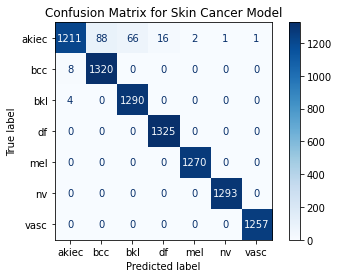
\includegraphics[width=\textwidth]{confusion_matrix.jpg} \caption{Confusion Matrix for Ensemble Learning Model} \label{fig } \end{figure}

% Additionally, a Receiver Operating Characteristic (ROC) curve was plotted for each class to evaluate the models' discrimination ability. The ensemble model exhibited a higher Area Under the Curve (AUC) for all classes, further confirming its superior performance.

\section{References}
\begin{thebibliography}{99}

\bibitem{Popescu2022} Popescu D., El-Khatib M., El-Khatib H., Ichim L. New trends in melanoma detection using neural networks: A systematic review. \textit{Sensors}. 2022;22:496. doi: 10.3390/s22020496.

\bibitem{Esteva2017} Esteva A., Kuprel B., Novoa R., Ko J., Swetter S.M., Blau H.M., Thrun S. Dermatologist-level classification of skin cancer with deep neural networks. \textit{Nature}. 2017;542:115–118. doi: 10.1038/nature21056.

\bibitem{Akram2020} Akram T., Lodhi H.M.J., Naqvi S.R., Naeem S., Alhaisoni M., Ali M., Haider S.A., Qadri N.N. A multilevel features selection framework for skin lesion classification. \textit{Hum.-Cent. Comput. Inf. Sci.}. 2020;10:1–26. doi: 10.1186/s13673-020-00216-y.

\bibitem{Pomponiu2016} Pomponiu V., Nejati H., Cheung N.-M. Deepmole: Deep neural networks for skin mole lesion classification. \textit{IEEE International Conference on Image Processing (ICIP)}. 2016;pp. 2623–2627.

\bibitem{Almaraz-Damian2020} Almaraz-Damian J.-A., Ponomaryov V., Sadovnychiy S., Castillejos-Fernandez H. Melanoma and nevus skin lesion classification using handcraft and deep learning feature fusion via mutual information measures. \textit{Entropy}. 2020;22:484. doi: 10.3390/e22040484.

\bibitem{Al-masni2020} Al-masni M.A., Kim D.-H., Kim T.-S. Multiple skin lesions diagnostics via integrated deep convolutional networks for segmentation and classification. \textit{Comput. Methods Programs Biomed.} 2020;190:105351. doi: 10.1016/j.cmpb.2020.105351.

\bibitem{Ichim2020} Ichim L., Popescu D. Melanoma detection using an objective system based on multiple connected neural networks. \textit{IEEE Access}. 2020;8:179189–179202. doi: 10.1109/ACCESS.2020.3028248.

\bibitem{Gong2020} Gong A., Yao X., Lin W. Classification for dermoscopy images using convolutional neural networks based on the ensemble of individual advantage and group decision. \textit{IEEE Access}. 2020;8:155337–155351. doi: 10.1109/ACCESS.2020.3019210.

\end{thebibliography}

\end{document}